% Slides centred on the package: every number comes from ../results/tables/numbers.tex.
% Structure adaptable: the forcing-maps slide can be skipped if time is short.

\begin{frame}
\titlepage
\vfill
\centering\scriptsize EarthFlux \EarthFluxVersion{} · \url{https://github.com/djwillichile/EarthFlux} · DOI 10.5281/zenodo.23981325
\end{frame}

\begin{frame}{Problema: mapas de agua con elecciones invisibles}
\begin{columns}[T]
\begin{column}{0.55\textwidth}
\begin{itemize}
  \item La evapotranspiración real ($\ETa$) mide el \textbf{uso consuntivo} del agua: insumo de balances hídricos, fiscalización y evaluación de riego.
  \item METRIC la estima con satélites y una calibración interna\ldots
  \item \ldots pero sus elecciones de entrada \textbf{rara vez se declaran}. La más común: \textbf{una sola estación} para toda la escena.
  \item Sin una herramienta que cambie esa elección dejando todo lo demás fijo, nadie sabe cuánto pesa.
\end{itemize}
\end{column}
\begin{column}{0.43\textwidth}
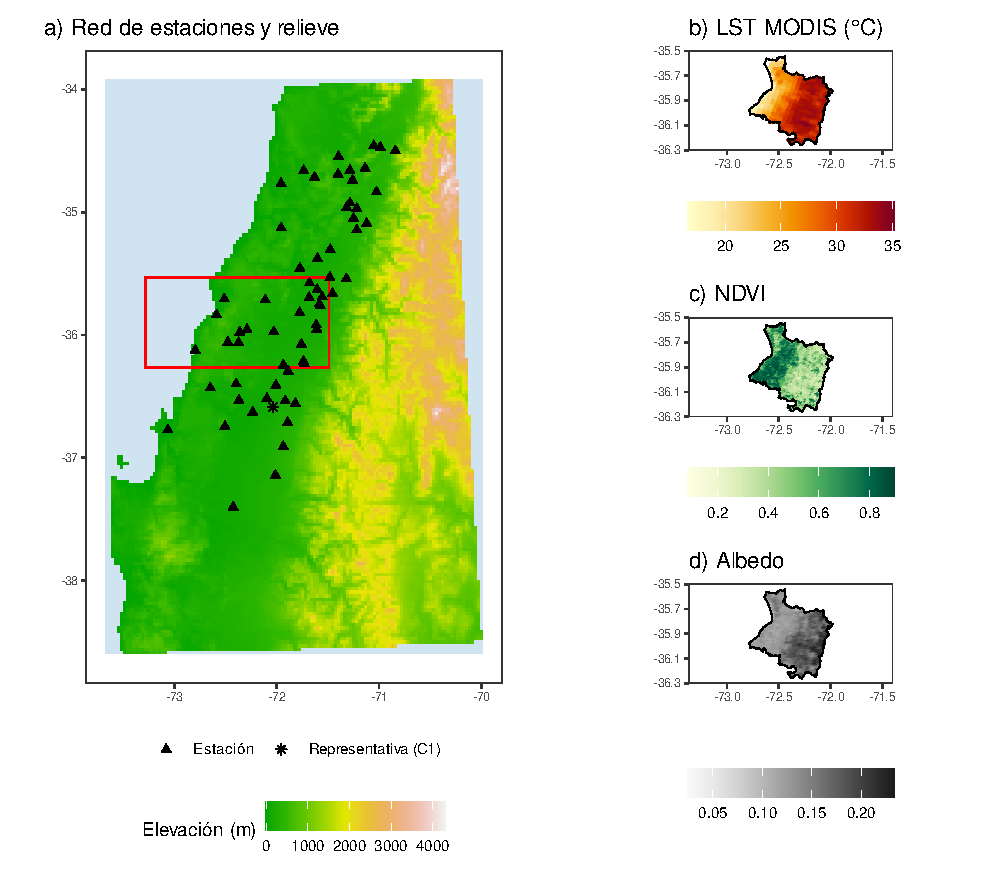
\includegraphics[width=\textwidth]{fig01_area.pdf}
\end{column}
\end{columns}
\end{frame}

\begin{frame}{EarthFlux: qué es y cómo está diseñado}
Paquete de R de código abierto (MIT) para flujos de energía y agua desde observaciones de la Tierra. Versión \EarthFluxVersion: \NExports{} funciones públicas, \NLinesR{} líneas de código R.
\vspace{3mm}
\begin{enumerate}
  \item \textbf{Física independiente del sensor}, con unidades documentadas.
  \item \textbf{Forzamiento intercambiable} bajo una sola interfaz: estación (C1), regresión global e IDW (C2), GWR (C3), con validación cruzada espacial.
  \item \textbf{Diagnósticos}: lo anómalo se marca, no se corrige en silencio.
  \item \textbf{Trazabilidad}: toda elección científica sin fuente única es explícita y queda registrada.
\end{enumerate}
\end{frame}

\begin{frame}{EarthFlux: verificación y estado}
\begin{columns}[T]
\begin{column}{0.5\textwidth}
\textbf{Verificado}
\begin{itemize}
  \item \VerVerified{} de \VerRows{} formulaciones coinciden con el manual de los autores del método; \VerDiscrepancies{} discrepancias halladas, \VerFixed{} corregidas.
  \item \NExpectations{} comprobaciones automáticas en cada revisión.
  \item Núcleo GWR = \pkg{GWmodel} hasta $10^{-10}$; secuencial = paralelo.
\end{itemize}
\end{column}
\begin{column}{0.47\textwidth}
\textbf{Aún experimental}
\begin{itemize}
  \item Sin flujo integrado que encadene todas las etapas.
  \item Sin descarga automática de escenas MODIS.
  \item Transmisividad y criterios de anclas: candidatos.
\end{itemize}
\end{column}
\end{columns}
\end{frame}

\begin{frame}{Caso de demostración: Cauquenes}
\textbf{¿Cuánto cambia la $\ETa$ si solo cambia el forzamiento meteorológico?}
\vspace{2mm}
\begin{itemize}
  \item MODIS, 15-02-2019 (\SceneCellsValid{} celdas de 1~km); \NStations{} estaciones públicas (DMC, INIA, FDF, NOAA).
  \item Cinco configuraciones con las \textbf{mismas ecuaciones, criterios y anclas}.
  \item Regionalización evaluada fuera de muestra: validación cruzada espacial anidada en \NCVDays{} días.
  \item \NMC{} réplicas Monte Carlo para comparar con otras fuentes de incertidumbre.
\end{itemize}
\vspace{2mm}
\textcolor{gray}{Hipótesis: el forzamiento cambia la $\ETa$ (H1, H2); GWR depende de la red (H3); más complejidad no garantiza más exactitud (H4).}
\end{frame}

\begin{frame}{Resultado 1: el forzamiento cambia la $\ETa$, por la $\ETr$ diaria}
\begin{columns}[T]
\begin{column}{0.55\textwidth}
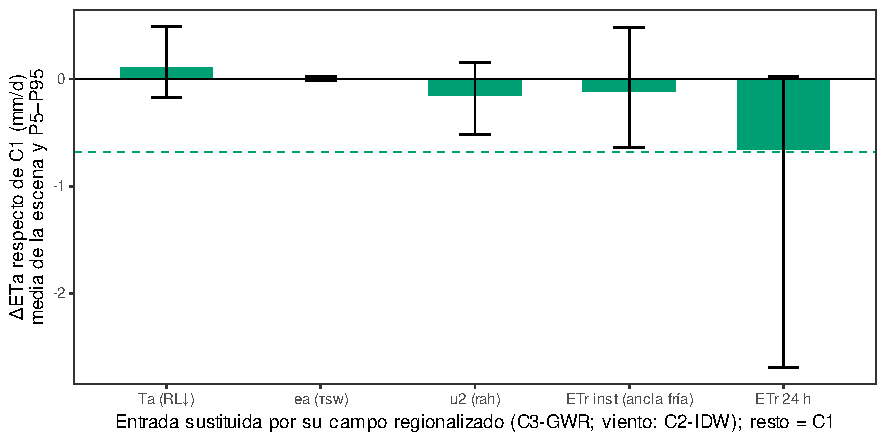
\includegraphics[width=\textwidth]{fig07_attribution.pdf}
\end{column}
\begin{column}{0.43\textwidth}
\small
\begin{itemize}
  \item $\ETa$ media: C1 \MEtaCOneMean{} → GWR \MEtaCThreeGWRMean{} mm/d (\textbf{\DEtaCThreeGWRPct\,\%}); IDW \DEtaCTwoIDWPct\,\%.
  \item $\ETrF$ casi no cambia (\DEtrfCThreeGWRPct\,\%): la calibración absorbe el forzamiento instantáneo.
  \item $\ETr^{24}$ sola: \DEtaOatEtrDayMean{} mm/d (H2).
\end{itemize}
\end{column}
\end{columns}
\end{frame}

\begin{frame}{Mapas de $\ETa$}
\centering
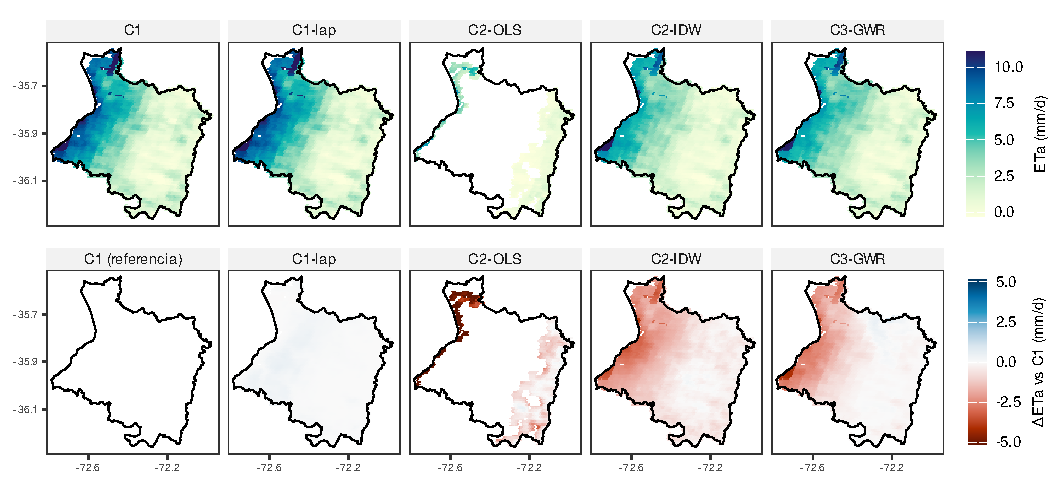
\includegraphics[width=\textwidth]{fig06_eta_maps.pdf}
\end{frame}

\begin{frame}{Resultado 2: el efecto es robusto}
\begin{columns}[T]
\begin{column}{0.55\textwidth}
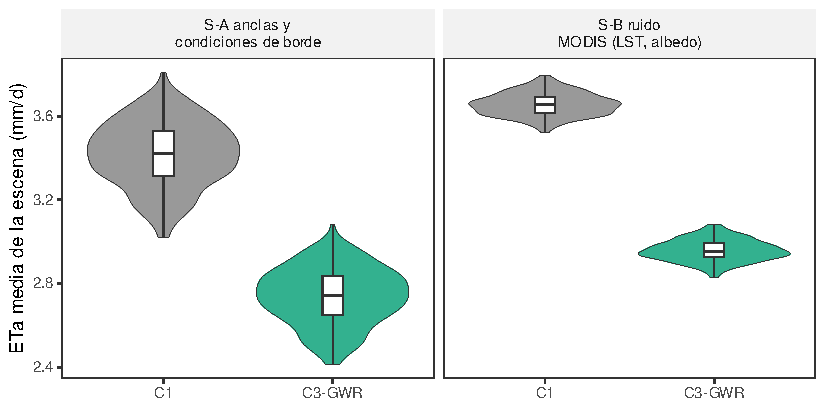
\includegraphics[width=\textwidth]{fig08_sensitivity.pdf}
\end{column}
\begin{column}{0.43\textwidth}
\small
\begin{itemize}
  \item Efecto GWR$-$C1: \SAEffMean{} mm/d, mismo signo en el \SAEffSign\,\% de las réplicas.
  \item \RatioSA{}× la dispersión por anclas y condiciones de borde.
  \item \RatioSB{}× la dispersión por ruido MODIS.
\end{itemize}
\end{column}
\end{columns}
\end{frame}

\begin{frame}{Resultado 3: la técnica más compleja no fue la mejor}
\begin{columns}[T]
\begin{column}{0.6\textwidth}
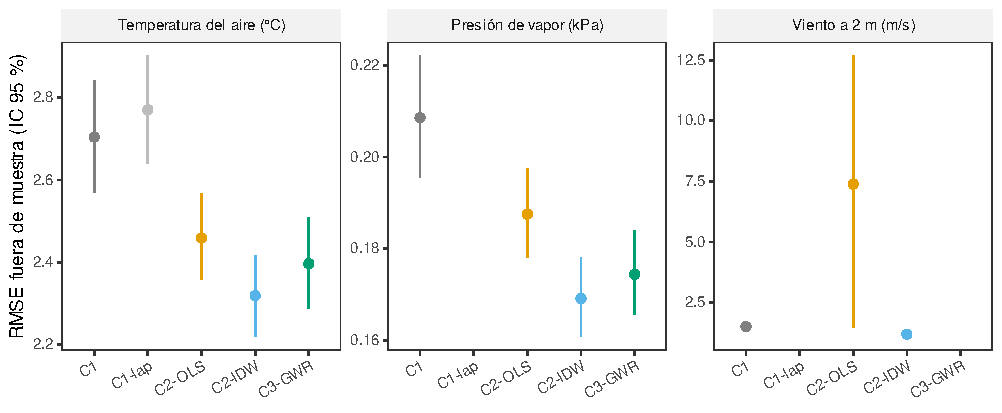
\includegraphics[width=\textwidth]{fig03_cv_rmse.pdf}
\end{column}
\begin{column}{0.38\textwidth}
\small
RMSE de $T_a$ (\si{\celsius}):\\
C1 \CVTaCOneRmse{} · OLS \CVTaCTwoOLSRmse{}\\
\textbf{GWR \CVTaCThreeGWRRmse{}} · \textbf{IDW \CVTaCTwoIDWRmse}
\begin{itemize}
  \item GWR $>$ C1 y OLS, pero \textbf{IDW $>$ GWR} (IC excluye 0).
  \item Viento: \NStationsWind{} estaciones $\Rightarrow$ GWR no factible.
\end{itemize}
\end{column}
\end{columns}
\end{frame}

\begin{frame}{Resultado 4: GWR depende de la red y extrapola}
\begin{columns}[T]
\begin{column}{0.55\textwidth}
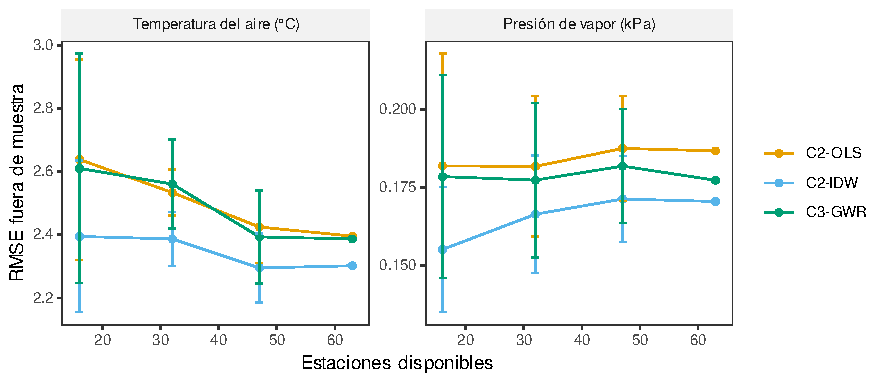
\includegraphics[width=\textwidth]{fig09_density.pdf}
\end{column}
\begin{column}{0.43\textwidth}
\small
\begin{itemize}
  \item 25\,\% de las estaciones: GWR \DensTaCThreeGWRQuarter{} \si{\celsius} frente a IDW \DensTaCTwoIDWQuarter.
  \item GWR supera el máximo observado (\RangeTaCThreeGWRObsMax~\si{\celsius}) en el \textbf{\RangeTaCThreeGWRAbove\,\%} de la escena, hasta \RangeTaCThreeGWRMax~\si{\celsius}.
  \item La validación cruzada en estaciones \textbf{no} detecta esto.
\end{itemize}
\end{column}
\end{columns}
\end{frame}

\begin{frame}{Campos meteorológicos a la hora del paso (H1)}
\centering
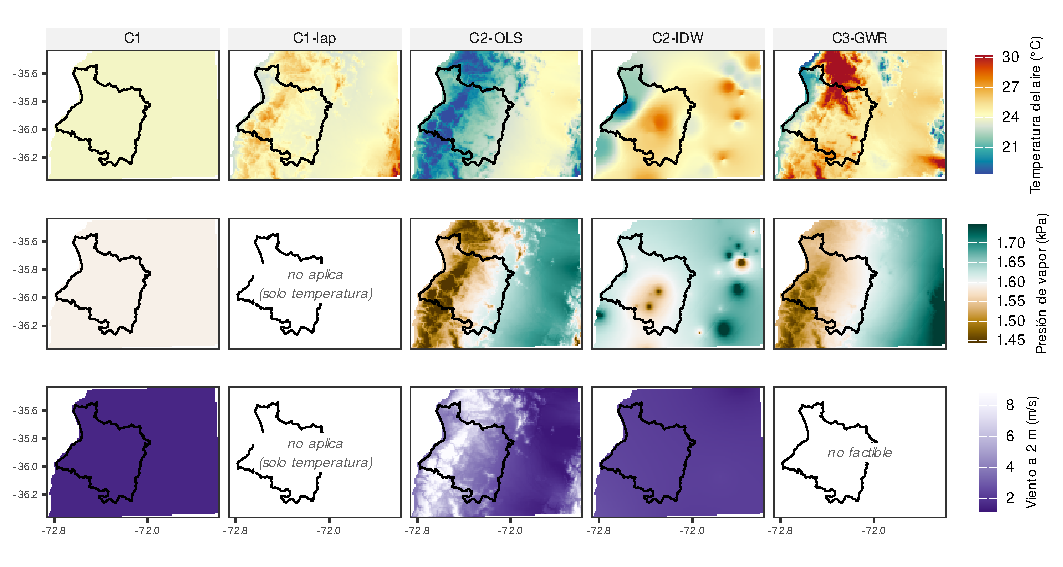
\includegraphics[height=0.82\textheight]{fig04_forcing_maps.pdf}
\end{frame}

\begin{frame}{Lo que el caso enseñó al paquete}
\begin{enumerate}
  \item \textbf{Flujo integrado}: hubo que encadenar unas veinte funciones a mano y declarar \NDecisions{} decisiones.
  \item \textbf{Múltiples escenas}: el estudio usó una sola, la que trae el paquete.
  \item \textbf{Diagnóstico de extrapolación de GWR}: la validación en estaciones no la detecta.
  \item \textbf{Validación con torres de flujo}.
\end{enumerate}
\vspace{3mm}
\textbf{Límites que no son del paquete, sino de los datos:} no hay mediciones públicas de flujos para la escena (exactitud de $\ETa$ no evaluada) y la red pública casi no mide viento ni radiación media.
\end{frame}

\begin{frame}{Implicaciones para la gestión hídrica}
\begin{itemize}
  \item La elección del forzamiento cambia la $\ETa$ entre \DEtaCThreeGWRPct{} y \DEtaCTwoIDWPct\,\%.
  \item En volumen: \VolDiffAbsCThreeGWR{} millones de m³ en \textbf{un solo día} ($\approx$\,\VolDiffFlowCThreeGWR~m³/s) entre GWR y C1. Desacuerdo entre modelos, no agua ahorrada.
  \item Pregunta de \textbf{valor de la información}: ¿cuánto cambia la estimación y por qué vía, antes de invertir en más datos?
  \item Los mapas de $\ETa$ usados en contabilidad o fiscalización deberían \textbf{declarar su forzamiento} y su sensibilidad.
  \item Las estaciones con viento y radiación en el secano son una \textbf{inversión directa} en certidumbre.
  \item El software abierto y verificable reduce el costo de auditar.
\end{itemize}
\vspace{2mm}
\small\textcolor{gray}{No se traducen diferencias de $\ETa$ en ahorros ni en beneficios monetarios.}
\end{frame}

\begin{frame}{Conclusiones}
\begin{enumerate}
  \item EarthFlux hace \textbf{visible y auditable} una incertidumbre que hoy no se declara.
  \item En Cauquenes, la sola elección del forzamiento cambió la $\ETa$ entre \DEtaCThreeGWRPct{} y \DEtaCTwoIDWPct\,\% (\VolDiffAbsCThreeGWR{} millones de m³ en un día con GWR).
  \item El efecto entra por la $\ETr$ diaria; la calibración absorbe el resto.
  \item La técnica más compleja (GWR) \textbf{no} fue la mejor.
  \item Próximos pasos: flujo integrado, múltiples escenas y validación con flujos.
\end{enumerate}
\vfill
\centering\small Guillermo S. Fuentes-Jaque · gfuentesj@correo.uss.cl · \url{https://github.com/djwillichile/EarthFlux}
\end{frame}
